\documentclass[conference]{IEEEtran}

\usepackage{tikz}

% correct bad hyphenation here
\hyphenation{}

\begin{document}
	
	\title{Implementacija spletnega pajka}
	
	\author{Skupina \textbf{DOMACI-NJOKI}}
	
	\maketitle
	
	\begin{abstract}
		V seminarju bomo opisali našo implementacijo spletnega pajka.
	\end{abstract}
	
	\IEEEpeerreviewmaketitle
	
	\section{Uvod}
	
	Pajek je razdeljen na več medsebojno povezanih komponent.
	
	\begin{figure}[h]
		\centering
		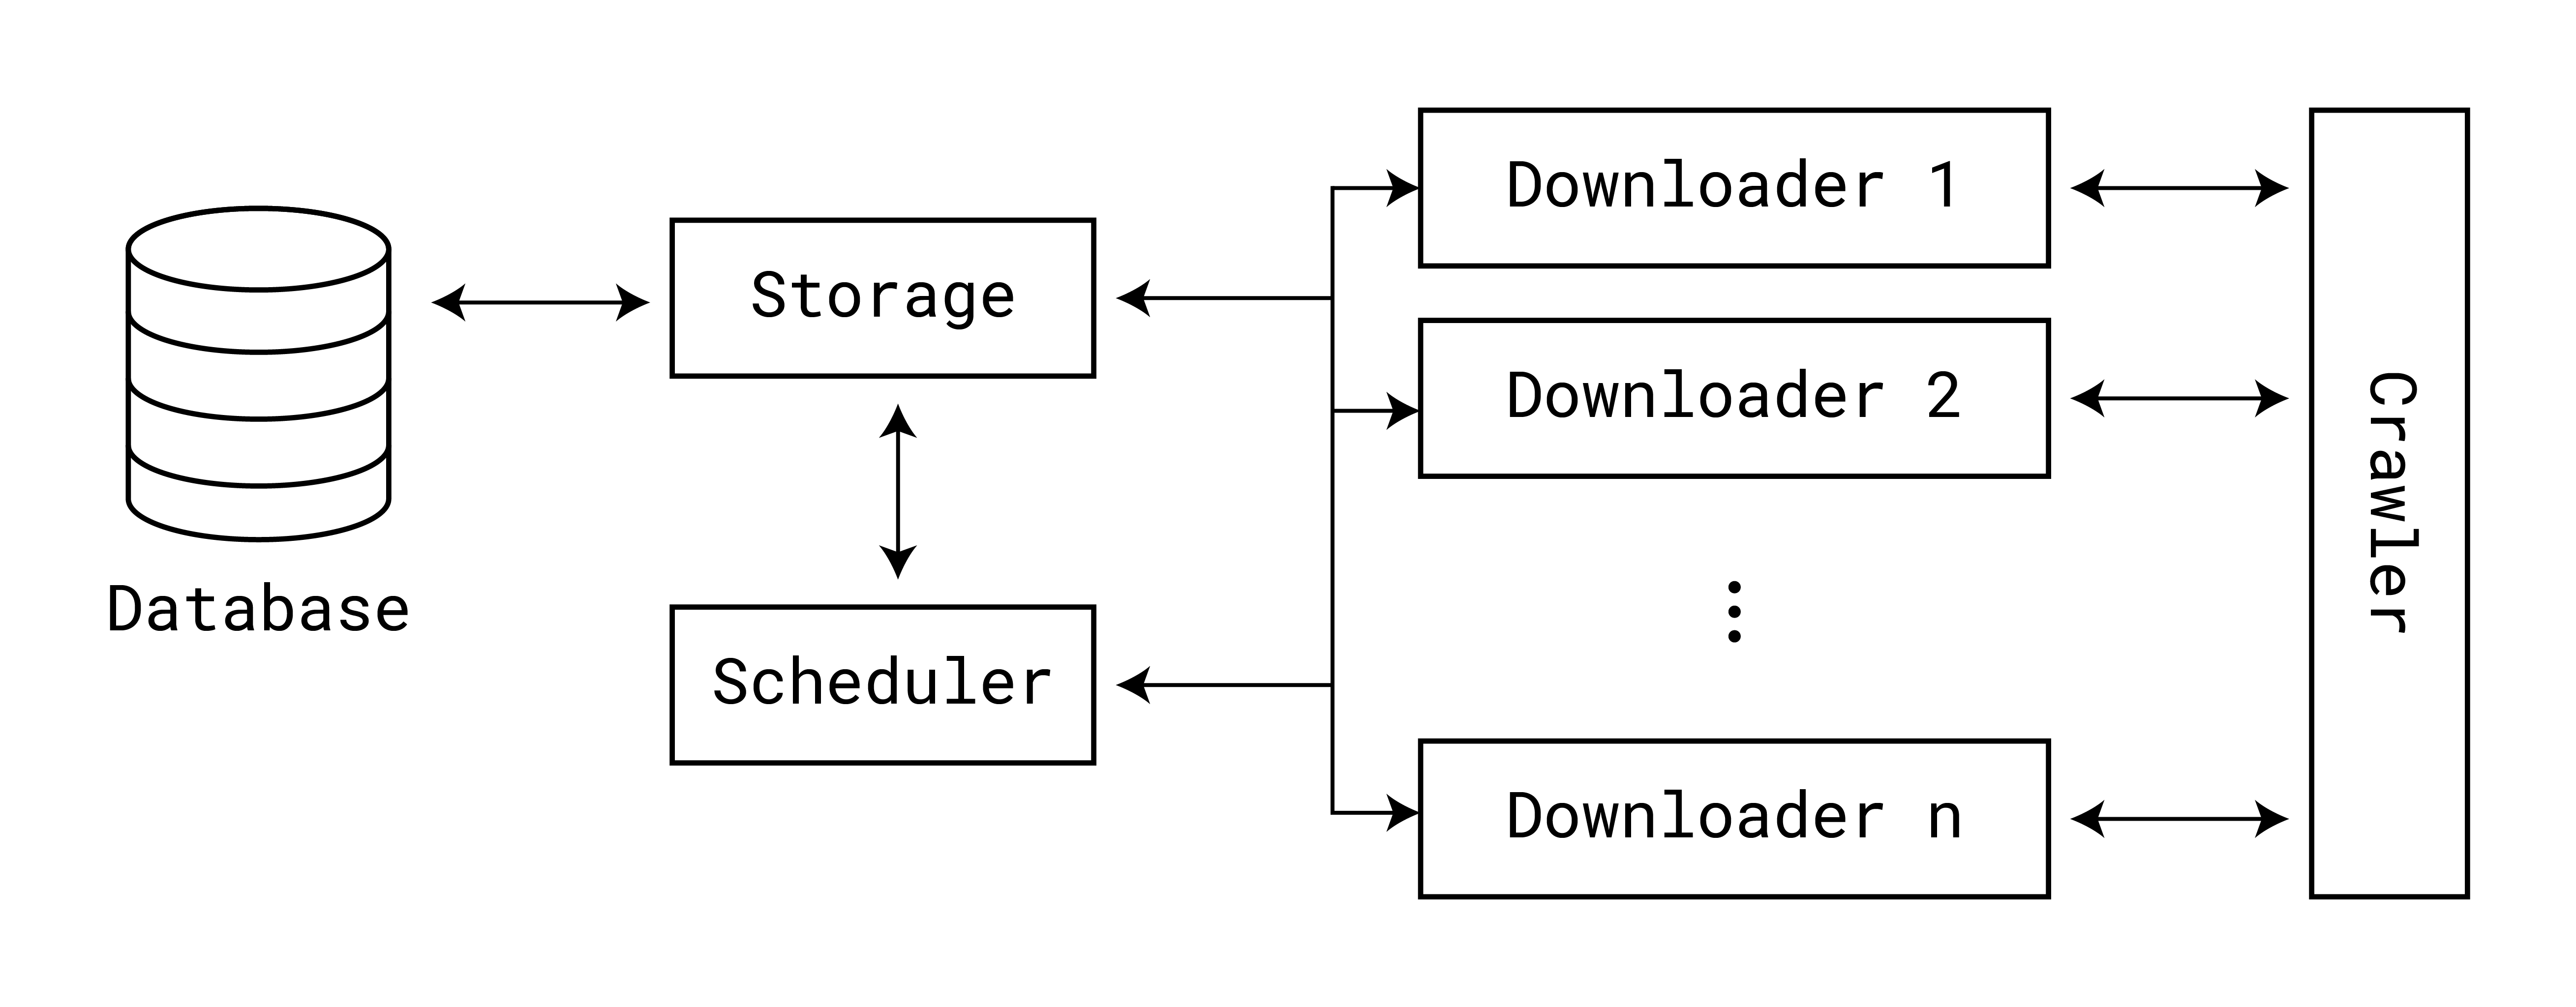
\includegraphics[width=.9\linewidth]{images/arhitecture}
		\caption{Arhitektura implementiranega spletnega pajka}
	\end{figure}

	\subsection{Razvrščevalnik}

	Razvrščevalnik (angl. scheduler) URL naslovov je implementiran kot podatkovna vrsta, do katere lahko obenem dostopa več različnih niti. 
	
	Ob dodajanju novega URL naslova v vrsto, razvrščevalnik preveri, ali je bil ta URL naslov že prenesen. Prav tako zna iz URL naslova prebrati domeno, pridobiti IP naslov strežnika s to domeno in prenesti datoteko \texttt{robots.txt}.
	
	\subsection{Pajek}
	
	Ob zagonu, pajek zažene več niti, vsaka od njih pa ima nalogo, da iz razvrščevalnika URL naslovov pridobi naslov, prenese stran in shrani podatke v podatkovno bazo. Pridobivanje vsebine strani izvajamo v dveh korakih:
	
	\begin{itemize}
		\item Najprej na strežnik izvedemo \texttt{HTTP HEAD} metodo.
		\item S pomočjo Selenium brskalnika obiščemo stran.
	\end{itemize}
	
	\subsection{Shramba}
	
	
	
	\section{Zaključek}
	
	% \bibliographystyle{IEEEtran}
	% \bibliography{}
	
\end{document}
